% Chapter Template

\chapter{Utilizzi del modello 3d in Odontoiatria} % Main chapter title

\label{Chapter6} % Change X to a consecutive number; for referencing this chapter elsewhere, use \ref{ChapterX}

 %----------------------------------------------------
 
 
Abbiamo discusso di come ottenere un modello 3d digitale dalle immagini diagnostiche e di come convertirlo in un modello fisico per mezzo della stampa 3D. Sia il modello digitale che il modello fisico sono elementi che possono elevare la qualità delle terapie fornite dal medico, ed allo stesso tempo sono di grande valore per il clinico ricercatore per la quantità di dati ottenibili.\\
I campi di applicazione sono molti ed abbracciano le discipline chirurgiche, l'educazione, procedure odontoiatriche quali l'implantologia, la protesi e la conservativa \parencite{Reference103}.
Discuteremo qui alcune delle implementazioni più rilevanti delle procedure che abbiamo descritto.

\section{Educazione}
\begin{wrapfigure} {R} {0.4\textwidth}
\vspace{-20pt}
	\begin{center}
	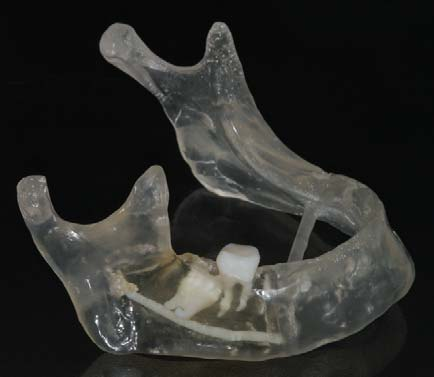
\includegraphics[width=0.4\textwidth, height=\textheight,keepaspectratio]{mandi_molar}
    \caption{modello3D ottenuto da CBCT, che presenta un terzo molare vicino al scondo molare, e con le radici in prossimità del nervo alveolare inferiore. Da \emph{Lambrecht et al} \parencite{Reference69}}
    \label{fig:mandi_molar}
    \end{center}
\vspace{-20pt}
\end{wrapfigure}
Nei corsi di laurea di ambito medico ed odontoiatrico il percorso di formazione del futuro professionista è un connubio di lezioni teoriche ed attività pratiche, volto a fornire delle approfondite conoscenze mediche ed un metodo di ragionamento clinico. Lo studente si trova soprattutto a dover sviluppare delle capacità manuali per eseguire degli interventi sul paziente.\\ Inoltre ogni studente in ambito sanitario studia l'\emph{anatomia}, e se un tempo le dissezioni su cadavere erano ciò che forniva agli studenti un contesto in cui applicare ciò che avevano appreso sui libri, ora sempre meno istituti offrono questa possibilità \parencite{Reference67}.\\
Con la diminuzione dell'uso dei cadaveri è aumentato l'utilizzo di repliche in plastica di parti dell'organismo come complemento pratico all'apprendimento dell'anatomia. Diversi autori hanno recentemente iniziato ad esplorare le possibilità offerte dalle moderne tecniche modellazione medica e stampa 3d nell'ambito della formazione medica.\\ Sono stati prodotti modelli anatomici e modelli per la spiegazione di procedure operative sia in ambito medico che odontoiatrico \parencite{Reference66}, \parencite{Reference70}. Heng \parencite{Reference67} ha valutato il miglioramento a breve termine in un test di conoscenza anatomica per gli studenti, dove venivano usati modelli di cuore stampati in 3d e cuori reali da cadavere, valutando positivamente l'esperienza con i modelli 3D. Lambrecht \parencite{Reference69} ha prodotto per mezzo di una stampante stereolitografica dei modelli di casi di chirurgia estrattiva per facilitare agli studenti l'apprendimento di procedure chirurgiche complesse \ref{fig:mandi_molar}.
\begin{figure}[h]
\vspace{-10pt}
	\begin{center}
	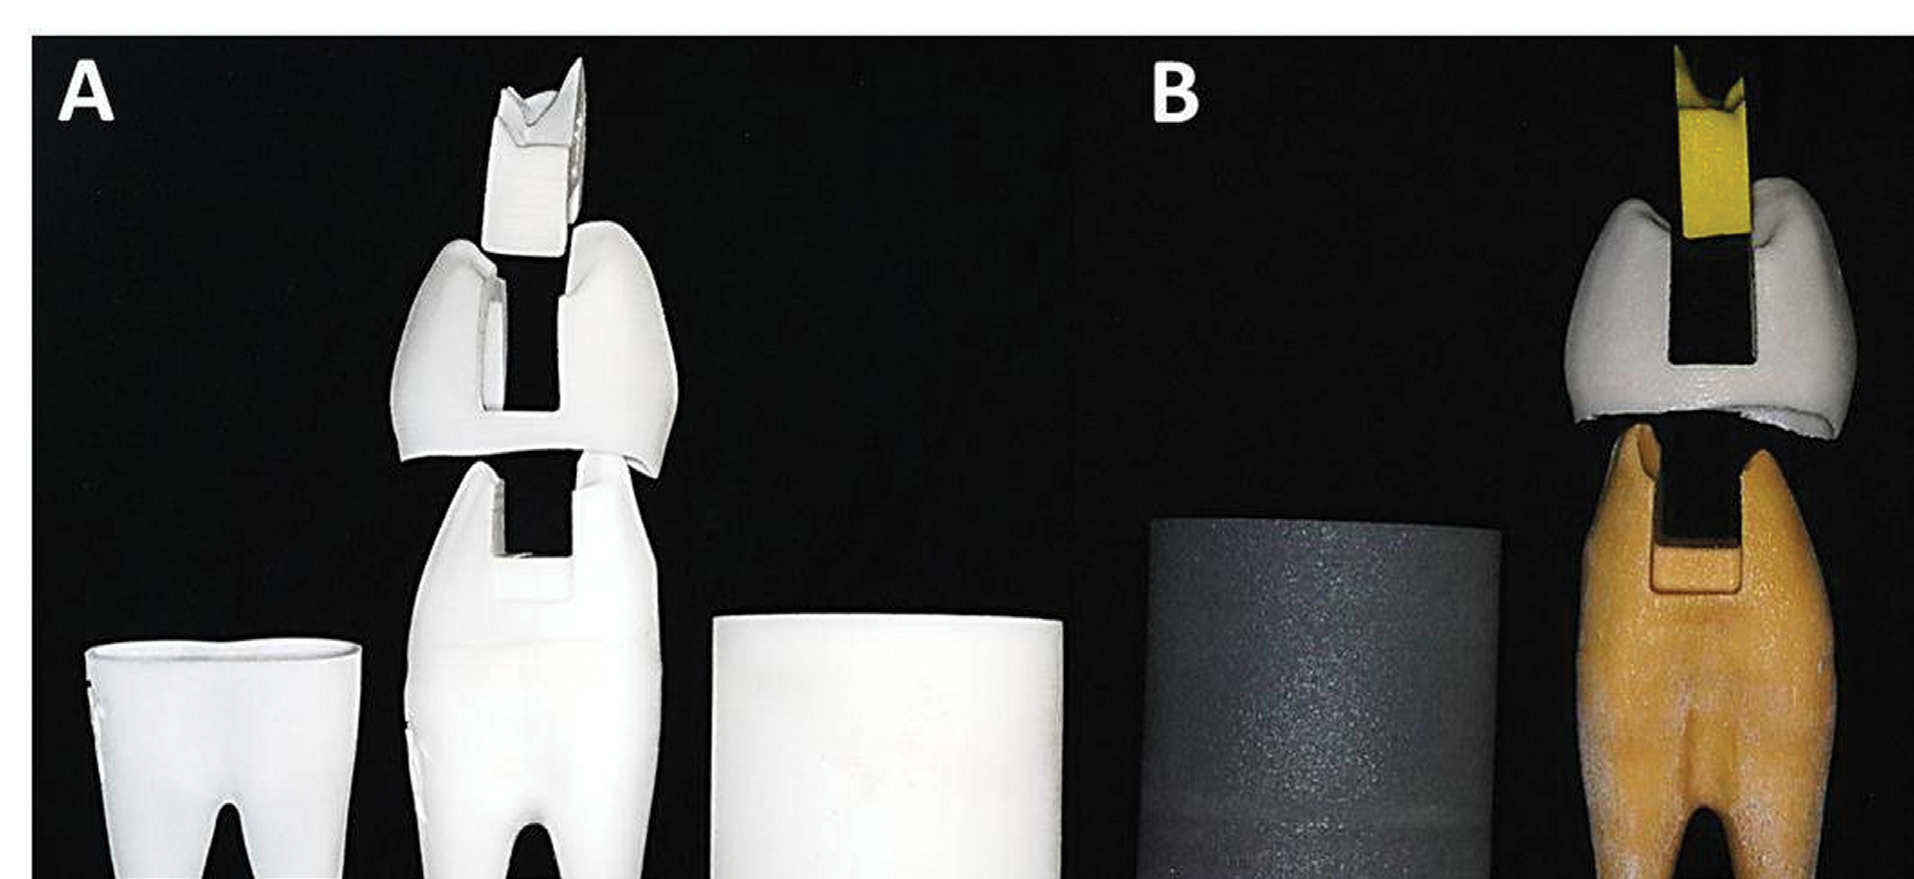
\includegraphics[width=0.8\textwidth, height=\textheight,keepaspectratio]{cavity_prep}
    \caption{Modelli dentali assemblabili rappresentanti delle preparazioni di cavità. Da \emph{Soares et al} \parencite{Reference71}}
    \label{fig:cavity_prep}
    \end{center}
\vspace{-20pt}
\end{figure}
\\ 
Soares et al \parencite{Reference71} ha prodotto modelli di elementi dentari preparati per istruire gli studenti sulle tecniche di preparazione di cavità \ref{fig:cavity_prep}. Altri autori hanno realizzato modelli 3d come supporto pratico ai corsi preclinici, ad esempio Kroger et al \parencite{Reference72} ha realizzato modelli per eseguire rimozioni di carie e realizzazione di provvisori; Reymus et al \parencite{Reference73} ha stampato repliche di elementi dentali con cavità endodontiche per simulare la preparazione endodontica. Il dato comune a questi studi era la valutazione generale positiva dei simulatori stampati in 3D si da parte degli studenti che dei docenti. Le stampanti 3d sono inoltre accolte con piacere dagli studenti e dal personale universitario, come documentato da Walker \parencite{Reference74}.\\
Sono già presenti online diverse librerie in cui è possibile trovare modelli anatomici, come quella fornita dal \emph{NIH} \parencite{Reference75} e quella presente sul sito web \emph{Embodi3d} \parencite{Reference76}. Inoltre le possibilità offerte dal flusso di lavoro qui descritto permettono di creare modelli anatomici originali di casi complessi o procedure particolari a costo ridotto. L'iniziale sforzo nell'uso dei software viene compensato dal ventaglio di possibilità offerte dal workflow in esame come ausilio all'educazione dell'odontoiatra in formazione.

\section{Programmazione dell'intervento chirurgico} 
La programmazione dell'intervento chirurgico è un passo importante per il trattamento del paziente, perché fornisce al team di chirurgia una conoscenza approfondita del caso in esame e permette di valutare l'approccio migliore alla chirurgia. Le tecniche di imaging digitale associate ai modelli 3D sono state sperimentate da diversi autori con l'obbiettivo di fornire al chirurgo un riferimento reale per programmare l'intervento.\\ Modelli che replicano l'anatomia della regione da operare sono stati creati per diverse chirurgie, dalla chirurgia vascolare alla chirurgia ortopedica. Il libro \emph{Medical Modeling} di Bibbs et al \parencite{Reference1} raccoglie una serie di interessanti casi clinici, chirurgici, odontoiatrici e di ricerca che mostrano utilizzo delle tecniche di modellazione medica e prototipazione rapida. Il chirurgo può simulare sui modelli l'esecuzione delle osteotomie, simulare la nuova disposizione dei segmenti ossei e creare guide chirurgiche come ausilio all'intervento \parencite{Reference77}, \parencite{Reference78}.
\begin{figure}[h]
\vspace{-10pt}
	\begin{center}
	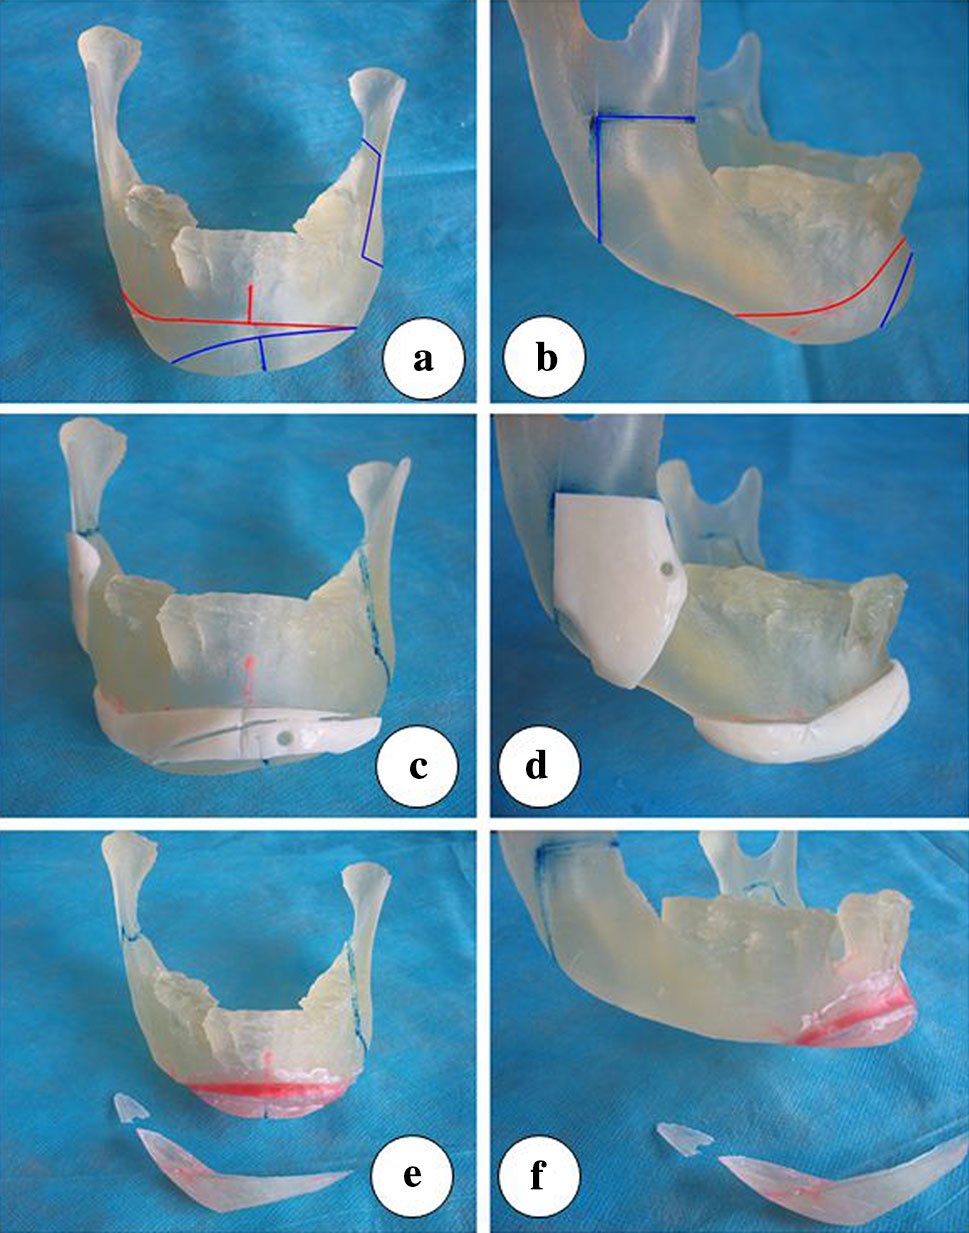
\includegraphics[width=0.5\textwidth,height=\textheight,keepaspectratio]{train_model}
    \caption{Modello per programmazione della chirurgia stampato in 3D.
\textbf{a}: Misure, analisi e linee di osteotomia marcate sul modello (vista frontale).\textbf{b}: Misure, analisi e linee di osteotomia marcate sul modello (vista laterale). \textbf{c}: Realizzazione del template chirurgico (vista frontale). \textbf{d}: Realizzazione del template chirurgico (vista laterale). \textbf{e}: Simulazione chirurgica (vista frontale). \textbf{f}: Simulazione chirurgica (vista laterale). Da \emph{Wang et al} \parencite{Reference20}.}
    \label{fig:train_model}
    \end{center}
\vspace{-20pt}
\end{figure}
\\ 
Ad esempio Wang \parencite{Reference109} ha riportato l'uso di modelli 3d per la programmazione della chirurgia ortognatica mandibolare e per la fabbricazione di guide chirurgiche, notando una maggior velocità e precisione nell'esecuzione dell'osteotomia e nel riposizionamento dei segmenti ossei \ref{fig:train_model}.\\
Il plugin di Blender \emph{OrtogOnBlender} \parencite{Reference64}, \parencite{Reference79} aiuta la programmazione dell'inter\-vento di \emph{chirurgia ortognatica} \ref{fig:ortogon1}, facilitando la simulazione delle osteotomie e permettendo di valutare le conseguenze delle mobilizzazioni ossee sul volto del paziente. Il viso del paziente può essere scannerizzato o rilevato con una serie di fotografie; OrtogOnBlender permette di ricavare modelli 3D attraverso la fotogrammetria, e di utilizzare questi modelli in combinazione con le scansioni TC per avvalersi dei modelli dell'interno e dell'esterno dell'orga\-nismo. In questo modo si possono simulare le conseguenze sul volto del paziente del riposizionamento dei segmenti ossei \parencite{Reference145}.
\begin{figure}[h]
\vspace{-10pt}
	\begin{center}
	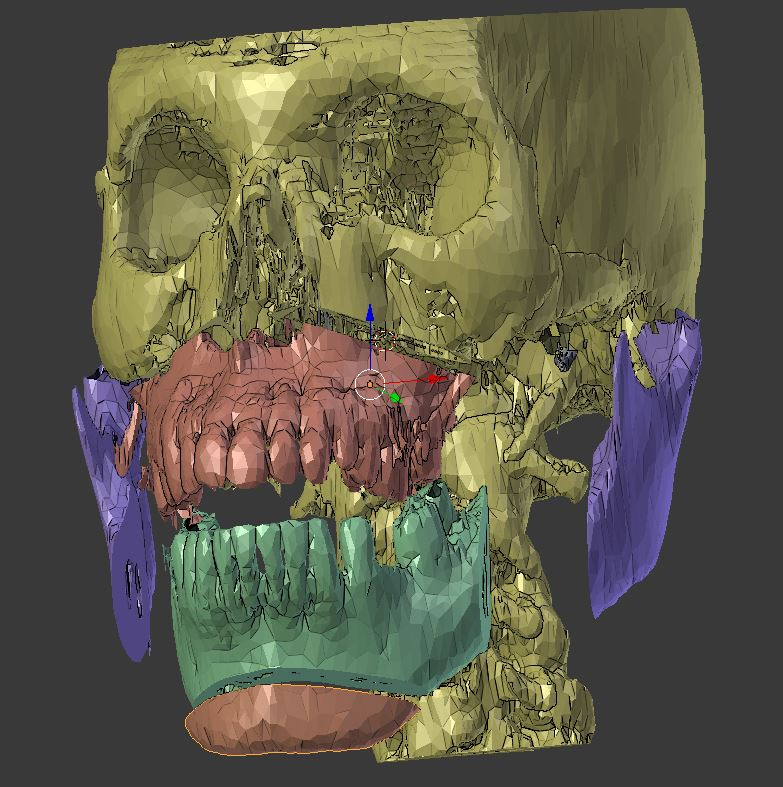
\includegraphics[width=0.6\textwidth,height=\textheight,keepaspectratio]{ortogon1}
    \caption{Osteotomie virtuali eseguite con add-on \emph{OrthogOnBlender}}
    \label{fig:ortogon1}
    \end{center}
\vspace{-20pt}
\end{figure}
\\
La procedura per la preparazione alla simulazione della chirurgia ortognatica con OrtogOnBlender \parencite{Reference80} consiste nel caricamento delle immagini DICOM in Blender, ma può essere utilizzato anche un modello .stl già processato. Il plugin facilità l'effettuazione delle osteotomie digitali mettendo a disposizione dei piani di taglio che vanno posizionati nella posizione desiderata; eseguite le osteotomie digitali possiamo isolare i segmenti e riposizionarli.\\
La gestione delle foto per la ricostruzione in fotogrammetria è molto agevole, basta importare la cartella contenente le foto ed il software automaticamente crea il modello del volto del paziente. Tramite poche operazioni la scansione del viso si allinea con le immagini della TC ed è possibile così la valutazione virtuale della ricollocazione dei mascellari.\\
Le tecnologie di prototipazione rapida sono state usate con successo per la realizzazione di un otturatore chirurgico personalizzato in seguito della rimozione di un carcinoma al mascellare superiore \parencite{Reference81}. \\
Ackland et al \parencite{Reference82} hanno riabilitato di una paziente con artrosi all'\emph{Articolazione Temporo Mandibolare} (ATM) disegnando una protesi personalizzata, sulla quale hanno eseguito simulazioni meccaniche al computer (FEA) per ottimizzarne la posizione ed il fissaggio. Il modello digitale è stato poi stampato in Titanio 6Al4V con una stampante SLS ed impiantato sulla paziente con buoni risultati.\\
L'integrazione delle tecniche digitali e della stampa 3D nel workflow chirurgico possono essere di notevole aiuto al chirurgo per la preparazione all'inter\-vento, soprattutto in casi di chirurgie complesse ed in aree delicate dell'organismo (ad esempio in prossimità di fasci neurovascolari). Queste tecnologie permettono inoltre di personalizzare eventuali dispositivi di riabilitazione, come protesi che si adattano all'anatomia ed alla biomeccanica del paziente. La collaborazione multidisciplinare nella programmazione chirurgica è un tassello portante di questo approccio riabilitativo incentrato sulla personalizzazione.


\section{L'odontoiatria digitale e la stampa 3D}
	
\subsection{Guide chirurgiche implantari}
L'imaging digitale è fondamentale in implantologia per la selezione del sito implantare, mentre le tecniche di modeling e prototipazione rapida permettono di creare velocemente delle guide chirurgiche personalizzate, che possono essere autoclavate ed utilizzate per l'inserimento degli impianti \parencite{Reference83}. Come mostrato da analisi della letteratura, la guida chirurgica permette di operare con maggior precisione rispetto alle procedure d'inserimento manuale dell'impianto. Van Assche \parencite{Reference105} ha effettuato una review della letteratura, dando indicazioni sull'utilizzo delle guide chirurgiche in implantologia (Fig. 34). La posizione dell'impianto inserito con le guide è più predicibile rispetto all'inserimento manuale, e la guida nella fase dell'inserimento dell'impianto ha una precisione maggiore rispetto alla guida delle sole osteotomie, dove solo la preparazione del sito è guidata, mentre il successivo inserimento della fixture è manuale. L'errore medio riscontrato con le guide è di circa 1mm nella posizione d'ingresso, 1,3mm all'apice ed una differenza di angolazione di circa 4 gradi, anche se con una ampia variabilità tra gli studi analizzati.
\begin{figure}[h!]
 
\begin{subfigure}{0.5\textwidth}
\centering
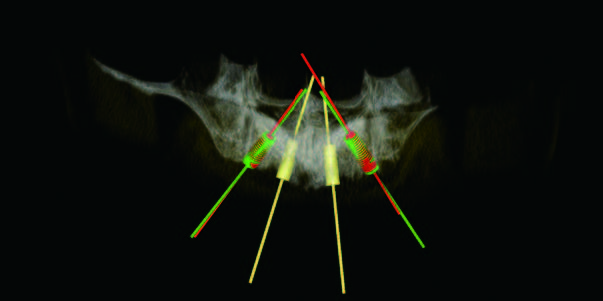
\includegraphics[width=0.9\linewidth, keepaspectratio]{beretta_digital} 
%\caption{Skirt}
\label{fig:beretta_digital}
\end{subfigure}
\begin{subfigure}{0.5\textwidth}
\centering
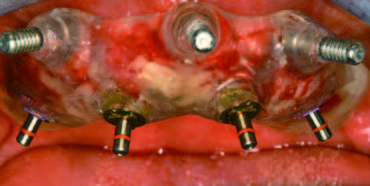
\includegraphics[width=0.9\linewidth, keepaspectratio]{beretta_real}
%\caption{}
\label{fig:beretta_real}
\end{subfigure}

 
\caption{\textbf{A sinistra}: Sovrapposizione tra simulazione degli impianti nella TC preoperatoria (rosso) e scansione postoperatoria con impianti inseriti (verde). \textbf{In basso}: Guida chirurgica per l'arcata madibolare, stabilizzata con miniimpianti. Da \emph{Beretta et al} \parencite{Reference104}.}
\label{fig:Beretta}
\end{figure}
\\
Beretta \parencite{Reference104} ha riscontrato dati simili in letteratura, ma nella sua piccola serie di 14 riabilitazioni implantari eseguite con guide chirurgiche ha trovato errori più bassi. La maggior precisione è da lui imputata ad alcuni accorgimenti, come l'uso di riferimenti extraorali per il corretto posizionamento anatomico, l'uso combinato di scansioni CT e scansioni ottiche nelle procedure di posizionamento, ed il fissaggio intraorale della guida con mini impianti \ref{fig:Beretta}.\\
Secondo i report analizzati l'utilizzo delle guide chirurgiche risulta un valido aiuto alle procedure d'inserimento implantare, tenendo presente un margine di errore adeguato di almeno 2mm da zone sensibili \parencite{Reference104}. L'accuratezza nella produzione delle guide è fondamentale, per cui si deve cercare di ridurre l'errore accumulato tra le operazioni di scansione delle arcate, di design e di manifattura della guida.
 

\subsection{Impianti Anatomici}
In campo implantologico degli autori hanno descritto impianti anatomici da inserire in alveoli postestrattivi (Root Analog Implant). Questi impianti sono realizzati con tecniche CAD/CAM di manifattura additiva o sottrattiva (fresatura), e replicano la morfologia dell'elemento dentario da sostituire. L'anatomia dell'alveolo può essere ottenuta mediante l'uso di una scansione CBCT oppure con la scansione ottica del dente estratto. La scansione ottica richiede di operare in due tempi, essendoci la necessità di estrarre il dente per scansionarlo, creare il modello digitale, stampare l'impianto e riaprire il sito chirurgico per inserirlo. La CBCT preoperatoria permette di pianificare l'intervento, creare l'impianto personalizzato per poi inserirlo subito dopo l'estrazione dell'elemento dentario, in un'unica seduta.
\begin{figure}[h]
\vspace{-10pt}
	\begin{center}
	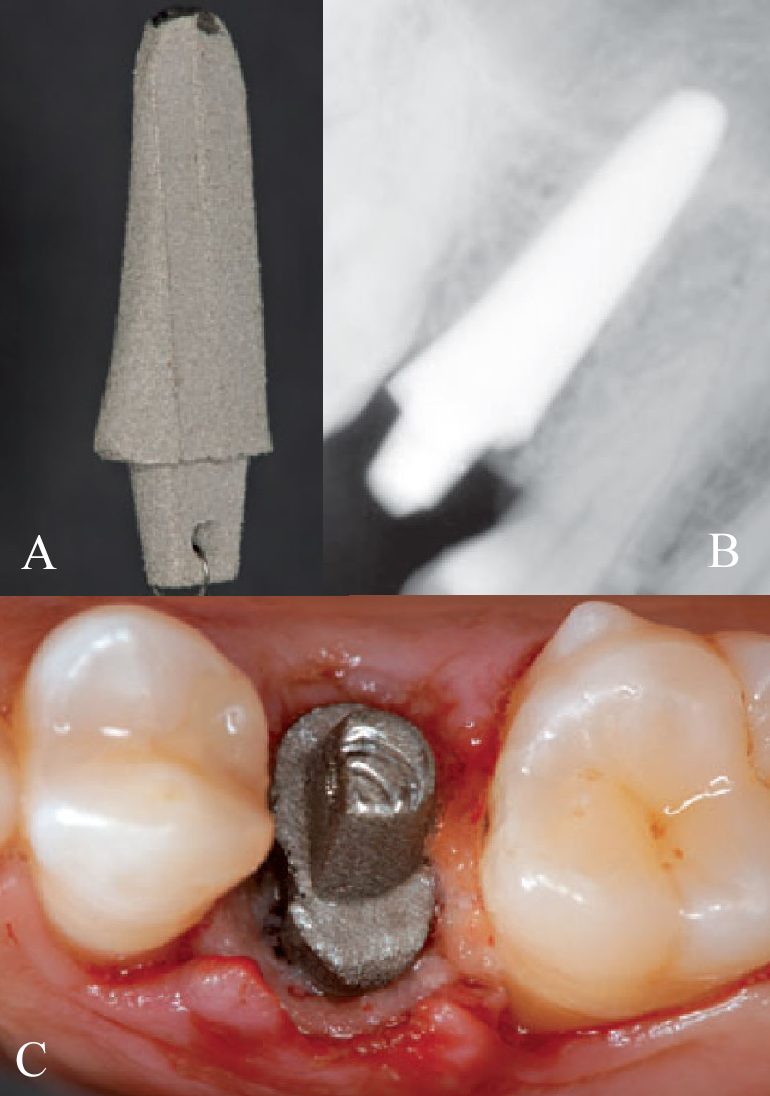
\includegraphics[width=0.5\textwidth,height=\textheight,keepaspectratio]{mangano_implant}
    \caption{Impianti anatomici realizzati con tecnologia DLMF. \textbf{A}: impianto anatomico in titanio. \textbf{B}: radiografia dell'impianto inserito in alveolo. \textbf{C}: aspetto clinico dell'impianto in cavo orale. Da \emph{Mangano et al} \parencite{Reference84}}
    \label{fig:mangano_implant}
    \end{center}
\vspace{-20pt}
\end{figure}
\\
Mangano \parencite{Reference84} ha utilizzato ricostruzioni CBCT per realizzare l'impianto personalizzato per mezzo della tecnologia di stampa DLMF (\emph{Direct Laser Metal Forming}), che usa un laser per sinterizzare layer di particelle di titanio dell'altezza di 0.2mm \ref{fig:mangano_implant}. L'impianto è stato protesizzato in maniera definitiva ed al controllo annuale si notava il mantenimento dei tessuti perimplantari.\\
Mangano \parencite{Reference85} ha poi eseguito uno studio su 15 pazienti, utilizzando impianti anatomici in titanio. Nonostante siano necessari ulteriori studi, il lavoro ha mostrato come gli impianti anatomici in titanio realizzati con tecnica DLMS (\emph{Direct Laser Metal Sintering}) possano essere una opzione di trattamento per casi di riabilitazione postestrattiva di elementi dentari in cui sia possibile una avulsione atraumatica, dove le corticali vengono mantenute intatte. \\
Pirker \parencite{Reference86} ha modificato la radice del dente estratto con l'aggiunta di macroritenzioni in composito sulla porzione distale e prossimale, lasciando inalterate la superficie vestibolare e la superficie linguale della radice. La radice così modificata è stata scansionata con uno scanner ottico, ed il modello digitale ottenuto è stato lievemente ridotto nel diametro della regione vestibolare e della regione linguale (tra 0.1 e 0.3 mm) per limitare il rischio di frattura delle corticali alveolari. L'impianto è stato poi prodotto in zirconia mediante un fresatore CAD-CAM ed impiantato nell'alveolo \ref{fig:bioimplant}. La stabilità primaria era ottimale, grazie all'uso delle macroritenzioni interdentali.  Al follow up a 2 anni non c'erano segni di riassorbimento osseo e retrazione gengivale, segno anche di una corretta distribuzione degli stress sulla parete dell'alveolo.
\begin{figure}[h]
\vspace{-10pt}
	\begin{center}
	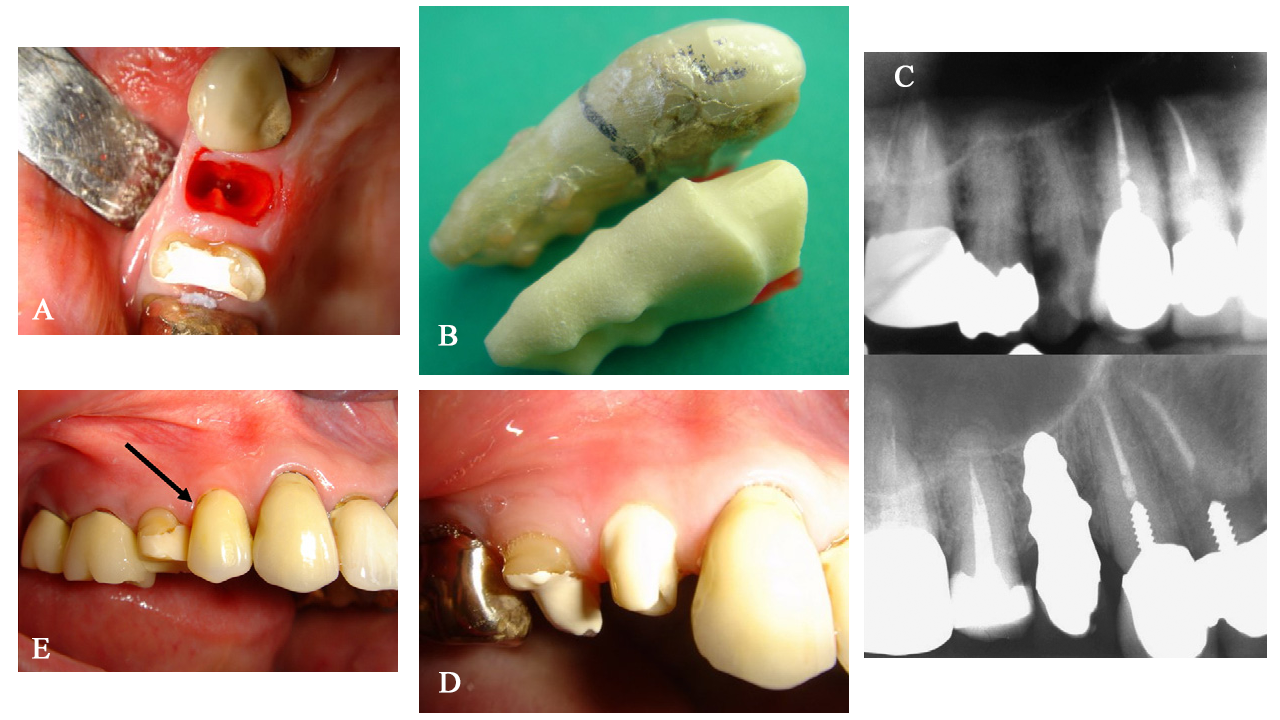
\includegraphics[width=0.9\textwidth,height=\textheight,keepaspectratio]{bioimplant}
    \caption{Inserimento e controllo impianto anatomico in zirconia. A: alveolo intatto di premolare estratto atraumaticamente. B: Elemento dentario estratto con ritenzioni simulate con composito, e impianto anatomico in zirconia con macroritenzioni. C: Radiografia pretrattamento (in alto) e post trattamento, con impianto anatomico inserito (in basso). D: impianto anatomico inserito. E: controllo clinico dopo 2 anni dall'inserimento dell'impianto; si nota il mantenimento dei tessuti parodontali. Da \emph{Pirker et al} \parencite{Reference86}}
    \label{fig:bioimplant}
    \end{center}
\vspace{-30pt}
\end{figure}
\\

Lo stesso autore ha poi effettuato una comparazione tra diverse topografie di impianti anatomici in zirconia realizzati con tecnologia CAD-CAM in un due gruppi di pazienti \parencite{Reference87}. Un gruppo di pazienti veniva riabilitato con impianti anatomici con una superficie rugosa realizzata mediante sabbiatura, mentre il secondo gruppo era trattato con impianti sabbiati su cui erano presenti macroritenzioni sulle superfici interdentali. Il gruppo di impianti sabbiati ha mostrato un tasso di successo dello 0\%, con tutti i 6 impianti inseriti che sono falliti prima di essere protesizzati. Il gruppo trattato con impianti con macroritenzioni ha mostrato un tasso di successo del 92\% a due anni, con solo un impianto perso su 12 inseriti. Il fallimento degli impianti con microritenzioni è stato imputato alla pressione uniforme esercitata dall'impianto sulle pareti dell'alveolo, mente ne caso con macroritenzioni la distribuzione del carico in aree definite ha permesso di ridurre lo stress sull'osso, favorendo l'osteointegrazione dell'impianto. \\
Patankar \parencite{Reference88} ha replicato la struttura anatomica in zirconia di Pirker con macroritenzioni interdentali, per la riabilitazione di un premolare inferiore, con un risultato positivo.\\

\begin{wrapfigure} {R} {0.4\textwidth}
\vspace{-20pt}
	\begin{center}
	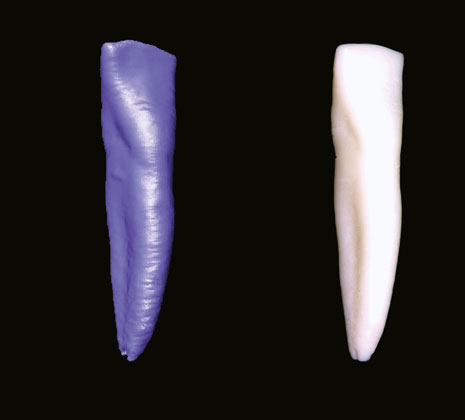
\includegraphics[width=0.4\textwidth, height=\textheight,keepaspectratio]{moin_dlp_zirconia}
    \caption{a sinistra modello CAD dell'elemento dentario. A destra modello dentario  in zirconia stampato stampato con tecnica DLP. Da \emph{Moin et al} \parencite{Reference89}}
    \label{fig:moin_dlp_zirconia}
    \end{center}
\vspace{-20pt}
\end{wrapfigure}

Moin \parencite{Reference89} ha utilizzato la tecnica di produzione additiva Digital Light Processing (DLP) per realizzare una replica in zirconia di un elemento dentale \ref{fig:moin_dlp_zirconia}. L'autore ha poi comparato digitalmente il modello CAD della replica, la scansione della replica stampata in zirconia e la scansione dell'elemento dentario originale, constatando l'adeguata precisione della tecnologia DLP per la fabbricazione additiva di manufatti in zirconia. \\
La produzione di manufatti in ceramica è attualmente possibile anche tramite la tecnica di stampa per estrusione, come documentato da Nötzel \parencite{Reference97}. Il processo usato consiste nella produzione di un filamento composto da paraffina, LDPE e particelle di Al2O3; il filamento viene stampato per estrusione a formare l'oggetto, che viene poi sottoposto a trattamento chimico e termico per la rimozione del medium in cui sono disperse le particelle di Al2O3 ed infine sinterizzato in forno a dare il manufatto finale. La stampa per estrusione di manufatti ceramici resta ancora da valutare nell'ambito della produzione di manufatti odontoiatrici. \\

Questi report ci dimostrano che, avvalendosi di tecniche digitali, la produzione di impianti anatomici è ormai possibile in maniera precisa e con l'utilizzo di biomateriali che favoriscono l'osteointegrazione ed una riabilitazione estetica e funzionale.\\
Importante risulta in quest'ottica la corretta determinazione della morfologia dell'alveolo e dell'impianto sostitutivo, e della distribuzione delle forze masticatorie sull'osso alveolare. Una avulsione atraumatica sta alla base della riabilitazione con impianti anatomici, perché eventuali traumi all'alveolo risultano in riassorbimenti ossei e retrazioni gengivali, con conseguente degradazione delle caratteristiche estetiche della riabilitazione. La distribuzione delle forze sull'alveolo è anch'essa da attenzionare.\\ Con gli impianti anatomici cerchiamo la stabilità primaria per mezzo della congruità dimensionale tra l'alveolo e l'impianto anatomico; è stato dimostrato che un eccessivo stress sulle pareti dell'alveolo causa il fallimento implantare, probabilmente per riduzione dell'apporto ematico al sito implantare ed all'osso circostante, che va incontro a riassorbimento. Ulteriori studi sono necessari per verificare la sicurezza e la standardizzazione delle procedure attualmente presenti, ma gli impianti anatomici potrebbero permettere, in casi selezionati, una soluzione funzionale ed estetica al problema del paziente, ed agevolare la risoluzione di casi di impianti postestrattivi mantenendo alti standard estetici.

\subsection{Protesi}
La prototipazione rapida è stata utilizzata sia in protesi fissa che in protesi rimovibile, per la realizzazione di restauri provvisori stampati, guide estetiche, mockup e per la realizzazione di scheletrati. Sono state usate varie tecnologie di manifattura additiva e vari materiali.\\
Tahayeri \parencite{Reference98} ha testato varie caratteristiche della stampa SLA con resine specifiche per l'uso dentale (NextDent), valutando l'influenza di alcuni parametri sulla precisione di stampa, sulle proprietà meccaniche e sul grado di conversione della resina. I provini stampati si sono dimostrati nel range di precisione richiesto per l'uso clinico, così come lo erano le proprietà meccaniche degli stessi campioni. L'autore ha notato differenze tra le caratteristiche nella stampa di varie resine dentali realizzate dallo stesso produttore, nonché differenti intensità del laser durante la polimerizzazione delle varie resine, in base al colore più o meno scuro della resina e del relativo tasso di assorbimento della luce. Una selezione di resine e stampanti ottimizzate per l'uso congiunto potrebbe migliorare ulteriormente la precisione di stampa; migliori risultati potrebbero derivare dalla fine regolazione delle caratteristiche della stampante in fase di stampa.
Da considerare che, secondo le indicazioni del produttore, la resina avrebbe dovuto subire un secondo passaggio di polimerizzazione dopo la stampa, cosa che gli autori non hanno eseguito per accelerare l'eventuale processo di produzione del provvisorio. Nonostante ciò le proprietà meccaniche della resina non post-polimerizzata si sono mostrate adeguate a resistere ai carichi intraorali. \\
Katreva \parencite{Reference99} ha realizzato un flusso di lavoro che ha integrato l'uso di modelli di lavoro stampati in 3D, la stampa 3D dei provvisori e la stampa della protesi definitiva per la conversione in ceramica pressata.\\
Revilla-León \parencite{Reference100} ha utilizzato un workflow digitale per la scansione delle impronte, la realizzazione della ceratura diagnostica, la stampa di una guida per la realizzazione dei provvisori ed infine per la produzione delle veneer, utili alla riabilitazione estetica e funzionale del settore anteriore dell'arcata mascellare. La guida per la realizzazione dei provvisori è stata realizzata mediante tecnica di stampa 3D DLP, mentre le veneer in disilicato di litio definitive sono state fresate al CAD-CAM.\\
Alharbi \parencite{Reference101} ha valutato la possibilità di realizzare corone protesiche con tecnica di stampa SLA. L'autore ha misurato l'accuratezza della corona stampata a varie angolazioni rispetto al piano e con l'uso di supporti di diverse dimensioni. Lo stesso gruppo di ricerca ha poi valutato l'accuratezza nella stampa di corone per mezzo della tecnica di stampa DLP \parencite{Reference102}. Entrambe le tecnologie si sono rivelate precise, con la stampa SLA che ha mostrato un maggior accuratezza nella replica della morfologia del modello digitale. Entrambe le tecnologie sono interessanti per l'impiego in odontoiatria, ma è necessario compiere ulteriori studi sull'influenza dei parametri di stampa sul modello finale ed approfondire le proprietà delle resine dentali.\\
\begin{wrapfigure} {R} {0.4\textwidth}
\vspace{-20pt}
	\begin{center}
	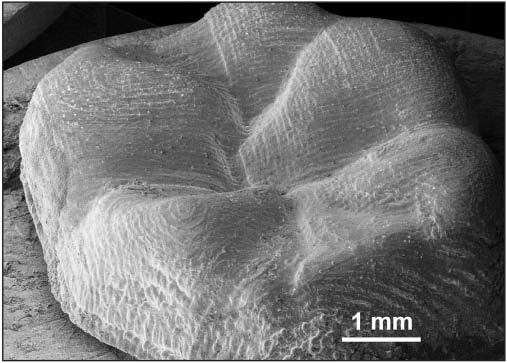
\includegraphics[width=0.4\textwidth, height=\textheight,keepaspectratio]{zircon_crown}
    \caption{Corona in zirconia realizzata con stampa ink-jet. Da \emph{Ebert et al} \parencite{Reference106}}
    \label{fig:zircon_crown}
    \end{center}
\vspace{-20pt}
\end{wrapfigure}

Ebert ha stampato corone in zirconia per mezzo di una stampante personalizzata, usando la tecnica ink-jet. Per realizzare la corona, una soluzione contenente zirconia veniva depositata strato dopo strato a formare il manufatto, che veniva poi sinterizzato in forno \ref{fig:zircon_crown}. Questo studio ha dimostrato che corone in zirconia con capacità meccaniche e precisione utili all'utilizzo clinico possono essere realizzate mediante tecnica di manifattura additiva ink-jet \parencite{Reference106}.\\
Alharbi \parencite{Reference107} ha valutato l'utilizzo della manifattura additiva in protesi, analizzando vari report e studi incentrati sulla protesi fissa e la protesi mobile parziale e totale. L'autore ha riportato che le sottostrutture metalliche realizzate con la metodica SLS (\emph{Selective Laser Sintering}) sono equivalenti o più precise rispetto alle procedure classiche di fusione per quanto riguarda il gap tra sottostruttura metallica e moncone dentale; allo stesso modo le proprietà meccaniche dei manufatti SLS erano equivalenti o migliori rispetto a quelli realizzati con le procedure classiche. Strutture metalliche per la realizzazione di protesi parziali rimovibili sono state prodotte per mezzo della manifattura additiva per via diretta o indiretta. La manifattura diretta consiste nella stampa del design per mezzo di processi SLS; la manifattura indiretta consiste nella realizzazione del manufatto in resina calcinabile per mezzo della stampa SLA oppure DLP, l'integrazione del modello calcinabile in materiale refrattario e la successiva colatura del metallo o della lega per la realizzazione del framework metallico. Entrambe le tecniche per la realizzazione dei framework per protesi removibile hanno mostrato una accuratezza accettabile, anche se i risultati derivano principalmente da studi in vitro e case report.\\
Lin \parencite{Reference108} ha dimostrato una tecnica per la realizzazione di protesi mobili totali provvisorie attraverso un protocollo digitale che prevede la scansione ottica, la ceratura diagnostica digitale della protesi, la stampa della base protesica e rispettiva arcata dentaria in fasi separate e con resine di colore e caratteristiche adatte, ed infine l'unione di arcata e base protesica \ref{fig:separ_full_prot}. Lo studio non ne ha testato l'uso sul paziente e non sono presenti ulteriori report della performance clinica di protesi mobili totali provvisorie realizzate con questa procedura e questi materiali. Questo concept potrebbe essere approfondito, valutando l'accuratezza rispetto agli altri metodi di fabbricazione disponibili e la durata della protesi nel tempo, sia dal punto di vista del colore che dell'usura della resina.\\
I dati disponibili sulle tecniche di programmazione digitale del trattamento e l'utilizzo delle tecnologie di manifattura additiva mostrano prospettive promettenti in odontoiatria, sia per la produzione di provvisori \parencite{Reference125} che di protesi removibili \parencite{Reference107}. Ulteriori studi e valutazioni con follow-up più lunghi sono comunque necessari prima di un'ampia applicazione clinica della tecnologia.  Resta inoltre poco esplorata la possibilità di produrre manufatti definitivi in ceramica o zirconia, possibilmente realizzabili con tecnologie come la SLS  o la stampa inkjet.
\begin{figure}[h]
\vspace{-10pt}
	\begin{center}
	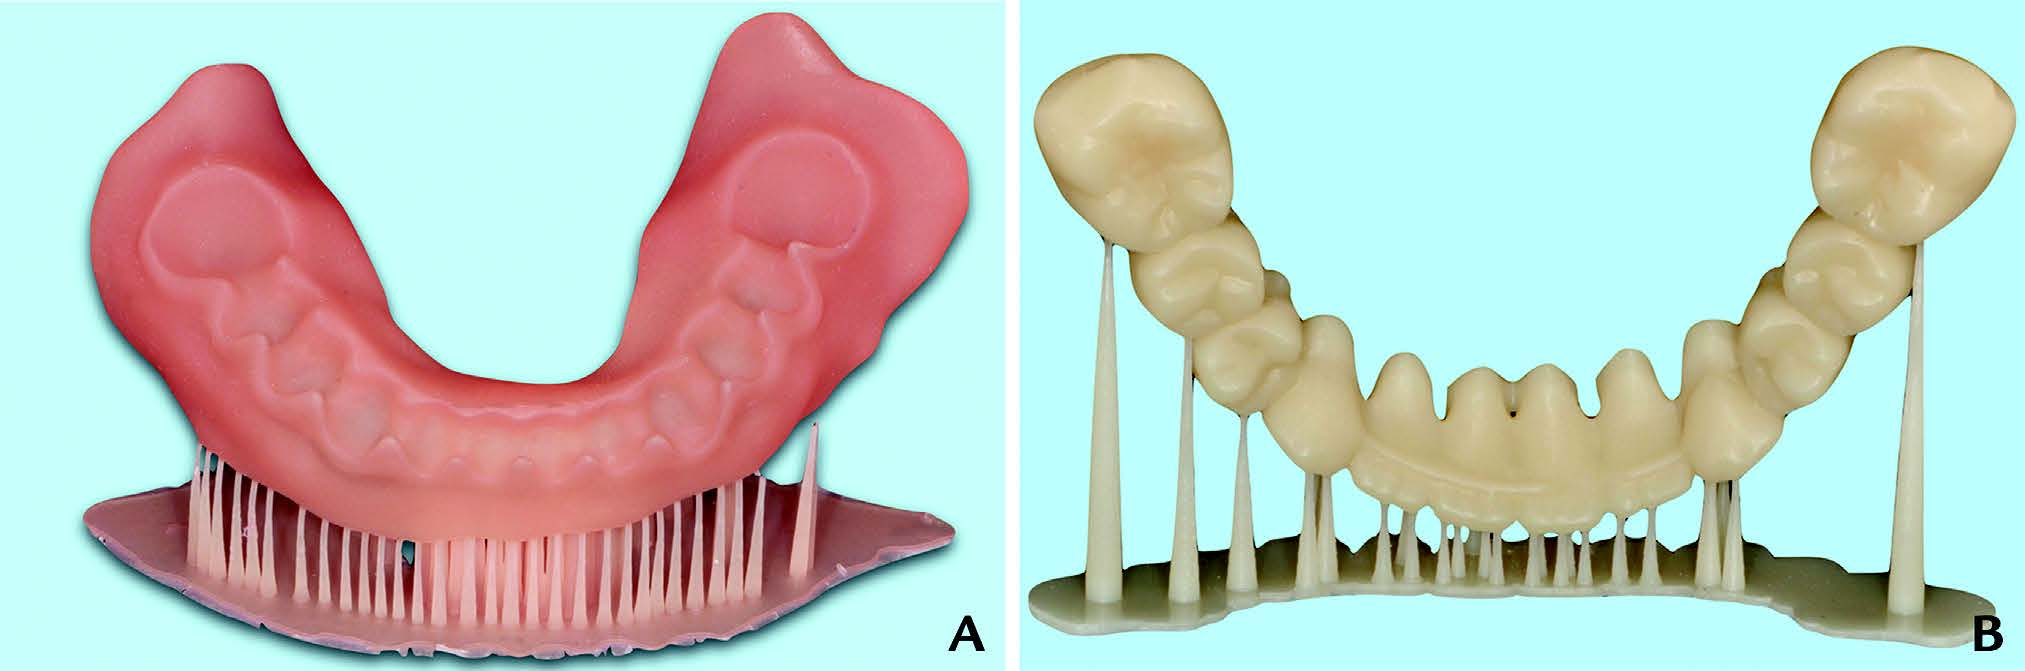
\includegraphics[width=0.9\textwidth,height=\textheight,keepaspectratio]{separ_full_prot}
    \caption{Componenti di Protesi mobile totale provvisoria realizzati con design digitale e stampante 3D DLP. Da \emph{Lin et al} \parencite{Reference108}}
    \label{fig:separ_full_prot}
    \end{center}
\vspace{-30pt}
\end{figure}

\subsection{Ortodonzia} 
L'ortodonzia è una delle branche dell'odontoiatria che più può avvalersi delle nuove possibilità di programmazione digitale del trattamento e dell'uso di tecnologie di manifattura additiva. La terapia ortodontica è classicamente programmata per mezzo di teleradiografie, modelli in gesso in articolatore e set di foto del paziente, oltre alla fondamentale valutazione clinica e funzionale. Le complesse relazioni tra le ossa del cranio coinvolte nella funzione orale sono difficilmente analizzabili in maniera adeguata su delle radiografie bidimensionali e con dei modelli in gesso, soprattutto se il trattamento prevede una fase chirurgica.\\
La terapia ortodontica digitale può avvalersi della possibilità di stampare brackets personalizzati \parencite{Reference115} e guide chirurgiche per l'inserimento di impianti ortodontici \parencite{Reference116} \ref{fig:stent_miniscrew}. La stampa 3d facilita anche la produzione di guide per il posizionamento dei brackets nel paziente \parencite{Reference127}, che favoriscono un posizionamento veloce e preciso degli stessi, e di strumenti ausiliari personalizzati \parencite{Reference126}. I brackets personalizzati sono stati realizzati da Krey attraverso il software FreeCAD ed un processo di stampa DLP \ref{fig:design_brackt}. Con la stessa tecnica è stato stampato uno splint di posizionamento, precedentemente progettato virtualmente, che ha permesso di posizionare i brackets in maniera rapida e precisa. Scansioni intraorali ad intervalli di tempo sono state effettuate e comparate in MeshLab per verificare lo spostamento ortodontico degli elementi dentali; anche lo splint di ritenzione post trattamento è stato progettato virtualmente e stampato in 3D.\\
\begin{figure}[h!]
 
\begin{subfigure}{0.5\textwidth}
\centering
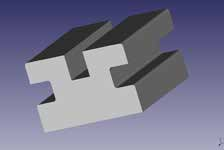
\includegraphics[width=0.9\linewidth, keepaspectratio]{design_brackt} 
\caption{Design CAD del bracket.}
\label{fig:design_brackt}
\end{subfigure}
\begin{subfigure}{0.5\textwidth}
\centering
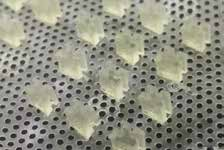
\includegraphics[width=0.9\linewidth, keepaspectratio]{printd_brackt}
\caption{Brackets stampati.}
\label{fig:printd_brackt}
\end{subfigure}
\begin{subfigure}{0.5\textwidth}
\centering
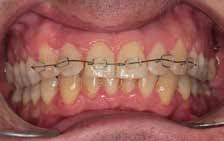
\includegraphics[width=0.9\linewidth, keepaspectratio]{working_brackt}
\caption{Brackets stampati in funzione all'interno del cavo orale.}
\label{fig:working_brackt}
\end{subfigure}
\begin{subfigure}{0.5\textwidth}
\centering
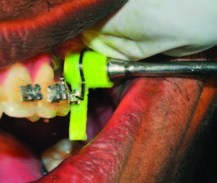
\includegraphics[width=0.7\linewidth, keepaspectratio]{stent_miniscrew}
\caption{Guida per l'inserimento di impianti ortodontici stampata in 3D}
\label{fig:stent_miniscrew}
\end{subfigure}
\caption{A, B e C da \emph{Krey et al} \parencite{Reference115}, D da \emph{Ahamed et al} \parencite{Reference116}}
\label{fig:3d_ortho}
\end{figure}


Questo è stato uno studio di prova con brackets \emph{edgewise} stampati in resina fotopolimerizzabile; gli autori hanno suggerito la possibiltà di rivedere parte del design per ottimizzare la resistenza dei brackets. Il report è in generale positivo e apre alla possibilità di un cambio radicale nel modo in cui l'ortodonzia con apparecchi fissi possa essere eseguita nello studio odontoiatrico, con il passaggio dall'uso di brackets generici a brackets personalizzati realizzabili in ambulatorio.\\
Nella moderna pratica odontoiatrica l'uso di modelli in gesso è spesso affiancato da scansioni digitali e dalla stampa 3d del modello. Diversi autori hanno valutato la precisione dei modelli realizzati con tecniche di manifattura additiva, con risultati diversi. Dietrich \parencite{Reference112} ha valutato la precisione e l'accuratezza di modelli dentali realizzati con stampa polyjet e con tecnica SLA. I modelli stampati sono stati scannerizzati e valutati via software per valutarne la discrepanza con l'originale. Entrambi i metodi di stampa si sono rivelati capaci di una accuratezza di stampa adeguata all'utilizzo ortodontico, con un errore massimo rilevato di circa \SI{100}{\micro\metre}.\\
Wan Hassan \parencite{Reference113} ha comparato manualmente, per mezzo di un calibro, modelli di arcate di pazienti con affollamento dentale, realizzati in gesso e stampati con tecnologia SLA. L'autore ha decretato i modelli non adatti all'uso ortodontico per via di una discrepanza di circa 1mm rispetto all'originale. L'autore riferisce che la scansione digitale dei modelli in gesso risultava in una perdita di dettaglio, inoltre le misurazioni con calibro risultavano a volte non semplici da effettuare per via dell'affollamento. Entrambe queste condizioni potrebbero aver contribuito all'errore riportato. Anche apparecchiature rimovibili possono essere fabbricate con la stampa 3d \parencite{Reference111}. Sono inoltre state usate guide chirurgiche stampate in 3d per effettuare osteotomie corticali allo scopo di accelerare i movimenti ortodontici \parencite{Reference114}.\\
Di rilievo è la possibilità di integrazione che l'ortodonzia digitale ci permette anche dal punto di vista biomeccanico. L'uso di scansioni ottiche e CBCT permette di avere dettagliate informazioni sulla struttura del paziente. I movimenti ortodontici si basano su principi biologici e fisici, dove vengono utilizzate forze controllate per attivare il processo di rimodellamento osseo, il quale permette il movimento dell'elemento dentario. Questi fattori potrebbero essere indagati integrando i dati anatomici (ossa, muscoli, legamenti, organi) ed i dati funzionali (forza masticatoria, caratteristiche meccaniche dei tessuti e materiali coinvolti, range di movimento mandibolare...) per simulare in silico il trattamento, fornendo al paziente un trattamento personalizzato secondo le sue caratteristiche biologiche e di risposta \parencite{Reference110}, \parencite{Reference140}.
\begin{figure}[h]
\vspace{-10pt}
	\begin{center}
	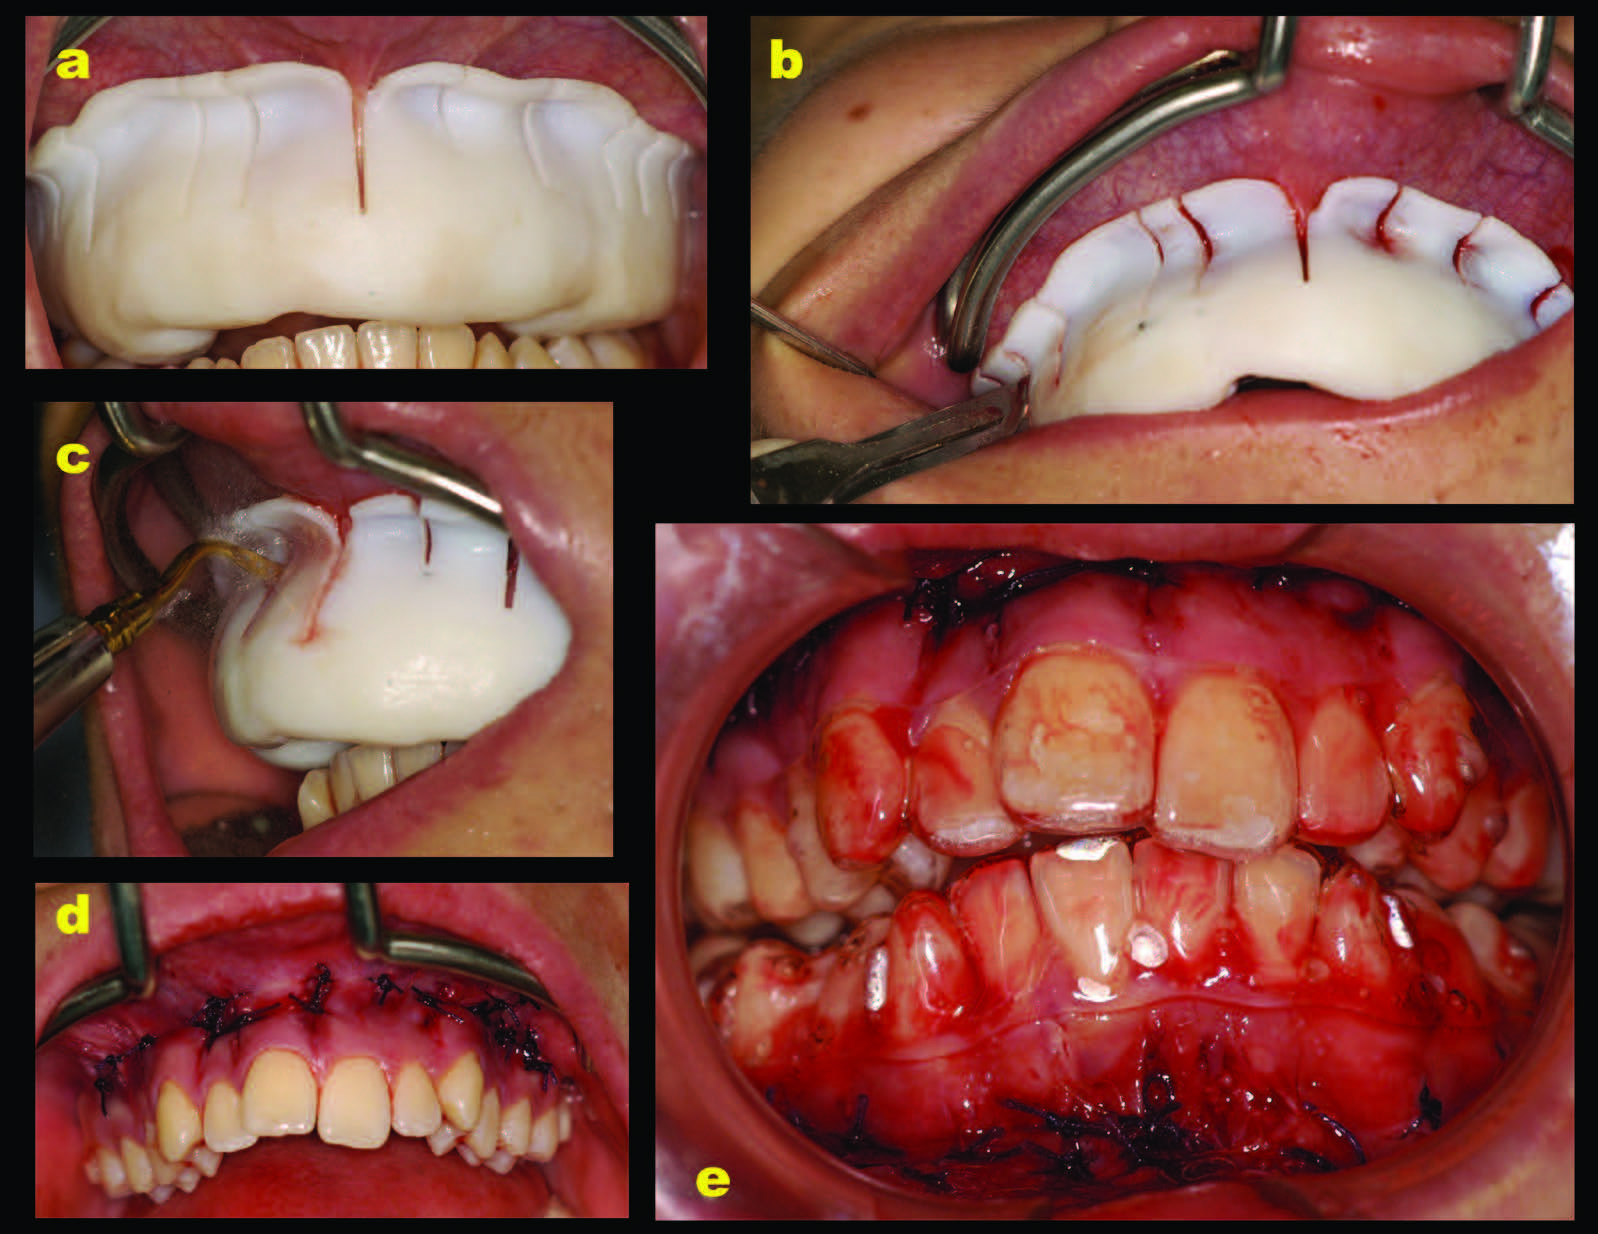
\includegraphics[width=0.9\textwidth, keepaspectratio]{guide}
    \caption{Posizionamento della guida chirurgica stampata in 3D per l'esecuzione di osteotomie flapless. \textbf{a}: Valutazione della stabilità intraorale. \textbf{b}: incisioni verticali della gengiva con bisturi n15. \textbf{c}: corticotomie verticali eseguite usando uno strumento piezoelettrico. \textbf{d}: sutura delle incisioni. \textbf{e}: posizionamento degli allineatori trasparenti dopo la chirurgia. Da \emph{Cassetta et al} \parencite{Reference114}.}
    \label{fig:guide}
	\end{center}
\vspace{-20pt}
\end{figure}

 
 